% ============================================================================
%  Parking Garage Management System — Technical Project Report
%  Compilable with: pdflatex report.tex  (run twice for ToC/refs)
% ============================================================================

\documentclass[12pt, a4paper]{report}

% ─────────────────────────── Packages ───────────────────────────
\usepackage[utf8]{inputenc}
\usepackage[T1]{fontenc}
\usepackage{lmodern}                     % Modern Latin font
\usepackage[margin=2.8cm]{geometry}      % Page margins (extra room for border)
\usepackage{graphicx}                    % Images
\usepackage{xcolor}                      % Colour support
\usepackage{hyperref}                    % Clickable links
\usepackage{listings}                    % Source-code listings
\usepackage{amsmath, amssymb}            % Math symbols
\usepackage{booktabs}                    % Professional tables
\usepackage{tabularx}                    % Full-width tables
\usepackage{caption}                     % Caption customisation
\usepackage{subcaption}                  % Sub-figures
\usepackage{enumitem}                    % List customisation
\usepackage{tikz}                        % Diagrams / page border
\usepackage{eso-pic}                     % Background on every page
\usepackage{fancyhdr}                    % Headers / footers
\usepackage{setspace}                    % Line spacing
\usepackage{parskip}                     % Paragraph spacing
\usepackage{float}                       % Float placement [H]
\usepackage{algorithm}                   % Algorithm floats
\usepackage{algpseudocode}               % Pseudocode
\usepackage{multicol}                    % Multi-column layouts
\usepackage[backend=biber,style=ieee]{biblatex} % Bibliography
\usepackage{microtype}                    % Better text justification

% ─────────────────── Page Border (every page) ───────────────────
\AddToShipoutPictureBG{%
  \begin{tikzpicture}[remember picture, overlay]
    \draw[black, line width=1.2pt]
      ([shift={(0.5cm,0.5cm)}]current page.south west)
      rectangle
      ([shift={(-0.5cm,-0.5cm)}]current page.north east);
  \end{tikzpicture}%
}

% ─────────────────── Overflow Prevention ────────────────────────
\sloppy                                   % Relax word spacing
\emergencystretch=1.5em                   % Extra stretch for tight lines
\setlength{\parskip}{0.5em}

% ─────────────────── Hyperref Configuration ─────────────────────
\hypersetup{
  colorlinks  = true,
  linkcolor   = black,
  citecolor   = blue!60!black,
  urlcolor    = blue!70!black,
  pdfauthor   = {Dhyey Joshi},
  pdftitle    = {Multi-Level Parking Garage Management System},
  pdfsubject  = {Data Structures Portfolio Project},
}

% ─────────────────── Code Listing Style ─────────────────────────
\definecolor{codebg}{HTML}{F5F5F5}
\definecolor{codeframe}{HTML}{CCCCCC}
\definecolor{codegreen}{HTML}{2E7D32}
\definecolor{codegray}{HTML}{757575}
\definecolor{codepurple}{HTML}{7B1FA2}
\definecolor{codeblue}{HTML}{1565C0}

\lstdefinestyle{cstyle}{
  language         = C,
  backgroundcolor  = \color{codebg},
  frame            = single,
  rulecolor        = \color{codeframe},
  basicstyle       = \footnotesize\ttfamily,
  keywordstyle     = \color{codeblue}\bfseries,
  commentstyle     = \color{codegreen}\itshape,
  stringstyle      = \color{codepurple},
  numberstyle      = \tiny\color{codegray},
  numbers          = left,
  numbersep        = 6pt,
  breaklines       = true,
  breakatwhitespace= false,
  columns          = flexible,
  showstringspaces = false,
  tabsize          = 4,
  captionpos       = b,
  xleftmargin      = 1.2em,
  framexleftmargin = 1.2em,
  xrightmargin     = 0.5em,
  aboveskip        = 1em,
  belowskip        = 0.8em,
}

\lstdefinestyle{pythonstyle}{
  language         = Python,
  backgroundcolor  = \color{codebg},
  frame            = single,
  rulecolor        = \color{codeframe},
  basicstyle       = \footnotesize\ttfamily,
  keywordstyle     = \color{codeblue}\bfseries,
  commentstyle     = \color{codegreen}\itshape,
  stringstyle      = \color{codepurple},
  numberstyle      = \tiny\color{codegray},
  numbers          = left,
  numbersep        = 6pt,
  breaklines       = true,
  breakatwhitespace= false,
  columns          = flexible,
  showstringspaces = false,
  tabsize          = 4,
  captionpos       = b,
  xleftmargin      = 1.2em,
  framexleftmargin = 1.2em,
  xrightmargin     = 0.5em,
}

\lstdefinestyle{jsstyle}{
  language         = Java, % Approximation for JS syntax
  backgroundcolor  = \color{codebg},
  frame            = single,
  rulecolor        = \color{codeframe},
  basicstyle       = \footnotesize\ttfamily,
  keywordstyle     = \color{codeblue}\bfseries,
  commentstyle     = \color{codegreen}\itshape,
  stringstyle      = \color{codepurple},
  numbers          = left,
  numbersep        = 6pt,
  breaklines       = true,
  breakatwhitespace= false,
  columns          = flexible,
  showstringspaces = false,
  tabsize          = 4,
  captionpos       = b,
  xleftmargin      = 1.2em,
  framexleftmargin = 1.2em,
  xrightmargin     = 0.5em,
  morekeywords     = {const, let, async, await, fetch, document},
}

\lstset{style=cstyle}

% ─────────────────── Headers and Footers ────────────────────────
\pagestyle{fancy}
\fancyhf{}
\fancyhead[L]{\small\nouppercase{\leftmark}}
\fancyhead[R]{\small Parking Garage}
\fancyfoot[C]{\thepage}
\renewcommand{\headrulewidth}{0.4pt}
\renewcommand{\footrulewidth}{0.4pt}

% ─────────────────── Line Spacing ───────────────────────────────
\onehalfspacing

% ─────────────────── Inline Bibliography ────────────────────────
% (Embedded references — no external .bib file required)
\addbibresource{\jobname.bib}

% We create an inline filecontents block so the document compiles standalone.
\begin{filecontents}{\jobname.bib}
@book{cormen2009,
  author    = {Thomas H. Cormen and Charles E. Leiserson and Ronald L. Rivest and Clifford Stein},
  title     = {Introduction to Algorithms},
  edition   = {3rd},
  publisher = {MIT Press},
  year      = {2009},
}
@book{kernighan1988,
  author    = {Brian W. Kernighan and Dennis M. Ritchie},
  title     = {The C Programming Language},
  edition   = {2nd},
  publisher = {Prentice Hall},
  year      = {1988},
}
@misc{flask2024,
  author    = {{Pallets Projects}},
  title     = {Flask --- A Python Microframework},
  year      = {2024},
  url       = {https://flask.palletsprojects.com/},
  note      = {Accessed: 2026},
}
@misc{djb2hash,
  author    = {Daniel J. Bernstein},
  title     = {Hash Function {DJB2}},
  year      = {1991},
  url       = {http://www.cse.yorku.ca/~oz/hash.html},
  note      = {Accessed: 2026},
}
@article{williams1964,
  author    = {J. W. J. Williams},
  title     = {Algorithm 232: Heapsort},
  journal   = {Communications of the ACM},
  volume    = {7},
  number    = {6},
  pages     = {347--349},
  year      = {1964},
}
@misc{mdn2024,
  author    = {{Mozilla Developer Network}},
  title     = {Fetch {API}},
  year      = {2024},
  url       = {https://developer.mozilla.org/en-US/docs/Web/API/Fetch_API},
  note      = {Accessed: 2026},
}
\end{filecontents}

% ════════════════════════════════════════════════════════════════
\begin{document}

% ======================= TITLE PAGE ============================
\begin{titlepage}
  \centering
  \vspace*{2cm}

  \rule{\textwidth}{1.5pt}\\[0.4cm]
  {\Huge\bfseries Multi-Level Parking Garage\\[0.3cm] Management System}\\[0.4cm]
  \rule{\textwidth}{1.5pt}\\[1.5cm]

  {\Large\textit{A Full-Stack Portfolio Project Demonstrating\\
  Hand-Rolled Data Structures in C\\
  with a Modern Web Frontend}}\\[2.5cm]

  {\large
  \begin{tabular}{r p{8cm}}
    \textbf{Author:}      & Dhyey Joshi \\[0.3cm]
    \textbf{Technologies:} & C~(Backend), Python/Flask~(Bridge), HTML/CSS/JS~(Frontend) \\[0.3cm]
    \textbf{Data Structures:} & Circular Queue, Min-Heap, Stack, Linked~List, Hash~Table \\[0.3cm]
    \textbf{Date:}         & \today \\
  \end{tabular}
  }

  \vfill
  {\small Repository: \texttt{parking-garage/}}
\end{titlepage}

% ====================== TABLE OF CONTENTS ======================
\tableofcontents
\newpage

% ====================== ABSTRACT ===============================
\chapter*{Abstract}
\addcontentsline{toc}{chapter}{Abstract}

This report presents the design, implementation, and testing of a
\textbf{Multi-Level Parking Garage Management System} --- a full-stack
application that manages parking slot allocation across three floors (60
total slots), handles VIP-prioritised waitlists, simulates a single-lane
exit (LIFO), maintains a chronological activity log, and computes
tiered billing with VIP discounts.

The backend is written entirely in~C without the C++ Standard Template
Library (STL); every data structure --- circular queue, min-heap priority
queue, linked-list stack, singly linked list, and hash table with
separate chaining --- is implemented from scratch.  A Python Flask
microserver bridges the backend to a glassmorphism-styled web frontend
via \texttt{subprocess} calls, enabling a clean separation of concerns
while keeping the architecture simple and educational.

The system passes 33~unit tests covering all data structures, and all
12~API endpoints have been verified end-to-end through the Flask
bridge.

% ====================== CHAPTER 1: INTRODUCTION ================
\chapter{Introduction}

\section{Problem Statement}

Urban parking facilities face several operational challenges:
\begin{itemize}[nosep]
  \item Efficiently allocating slots across multiple floors without
        linear scans.
  \item Prioritising reserved and VIP vehicles when the lot is full.
  \item Modelling physical constraints such as single-lane exits where
        only the last car in can leave first.
  \item Tracking vehicle locations for instant retrieval.
  \item Computing fair, tiered billing with promotional discounts.
\end{itemize}

This project addresses all five challenges by mapping each to a
classical data structure, making it both a practical system and an
educational showcase.

\section{Objectives}

\begin{enumerate}[nosep]
  \item Implement five core data structures from scratch in~C (no STL).
  \item Build a garage orchestration layer that ties all structures
        together with state persistence.
  \item Create a Python Flask bridge to connect the C backend to a web
        frontend via \texttt{subprocess}.
  \item Develop a responsive, glassmorphism-styled dashboard using
        vanilla HTML, CSS, and JavaScript.
  \item Verify correctness through unit tests and end-to-end API testing.
\end{enumerate}

\section{Scope}

The system manages a \textbf{3-floor garage with 20~slots per floor}
(60~total).  Configuration constants (\texttt{NUM\_FLOORS},
\texttt{SLOTS\_PER\_FLOOR}) are defined in a single header, making the
system easily scalable.

% ====================== CHAPTER 2: SYSTEM ARCHITECTURE ==========
\chapter{System Architecture}

\section{High-Level Design}

The application follows a three-tier architecture:

\begin{center}
\resizebox{0.92\textwidth}{!}{%
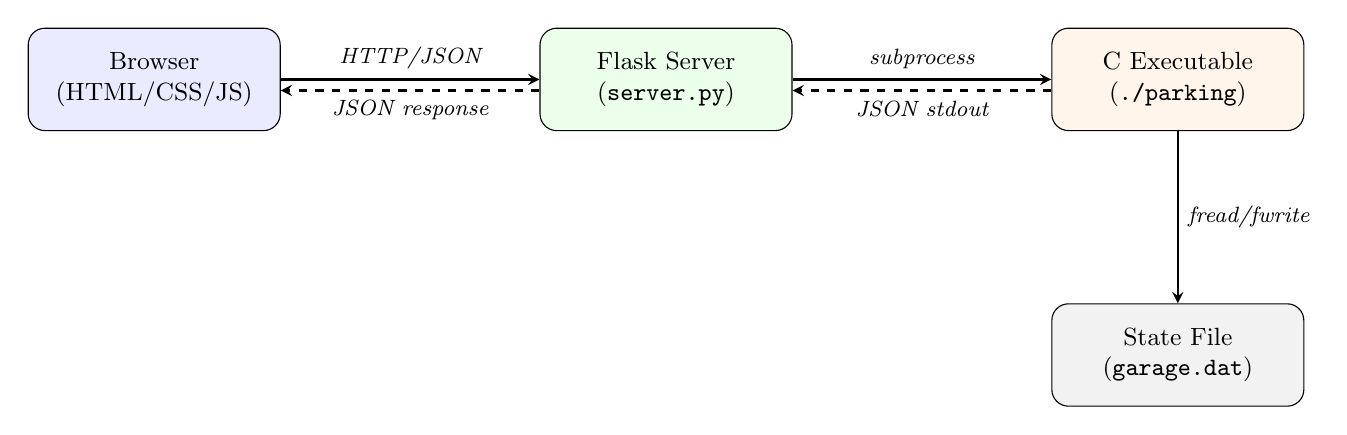
\begin{tikzpicture}[
  box/.style={draw, rounded corners=6pt, minimum width=3.2cm,
              minimum height=1.3cm, align=center, font=\small,
              inner sep=6pt},
  arrow/.style={->, >=stealth, thick},
]
  % Nodes — spread out for label breathing room
  \node[box, fill=blue!8]   (fe) at (0,0)     {Browser\\(HTML/CSS/JS)};
  \node[box, fill=green!8]  (fl) at (6.5,0)   {Flask Server\\(\texttt{server.py})};
  \node[box, fill=orange!8] (be) at (13,0)    {C Executable\\(\texttt{./parking})};
  \node[box, fill=gray!10]  (db) at (13,-3.5) {State File\\(\texttt{garage.dat})};

  % Forward arrows (above the line connecting boxes)
  \draw[arrow] (fe.east) -- node[above, font=\footnotesize\itshape] {HTTP/JSON} (fl.west);
  \draw[arrow] (fl.east) -- node[above, font=\footnotesize\itshape] {subprocess} (be.west);
  \draw[arrow] (be.south) -- node[right, font=\footnotesize\itshape] {fread/fwrite} (db.north);

  % Return arrows (offset below to avoid overlapping forward arrows)
  \draw[arrow, dashed] ([yshift=-4pt]be.west) -- node[below, font=\footnotesize\itshape] {JSON stdout} ([yshift=-4pt]fl.east);
  \draw[arrow, dashed] ([yshift=-4pt]fl.west) -- node[below, font=\footnotesize\itshape] {JSON response} ([yshift=-4pt]fe.east);
\end{tikzpicture}%
}% end resizebox
\end{center}

\section{Design Rationale}

\textbf{Why a subprocess bridge instead of sockets?}

The C program is intentionally \emph{stateless per invocation}: it loads
\texttt{garage.dat}, performs one operation, prints JSON to
\texttt{stdout}, and saves the state back.  Flask calls it via Python's
\texttt{subprocess.run()}, capturing \texttt{stdout} as the HTTP
response.  This approach:

\begin{itemize}[nosep]
  \item Keeps the C code free of networking, HTTP parsing, and
        thread-safety concerns.
  \item Makes debugging trivial --- the C executable works as a
        standalone CLI tool.
  \item Is simpler to learn than raw POSIX sockets or embedded HTTP
        servers.
\end{itemize}

\section{State Persistence}

The garage state is serialised to a binary file (\texttt{garage.dat})
using \texttt{fwrite}/\texttt{fread}.  The file begins with a 4-byte
magic number (\texttt{0x50415243}, ASCII ``PARC'') for validation.  Each
section is written sequentially:

\begin{enumerate}[nosep]
  \item Magic number + total revenue (cents).
  \item Per-floor circular queue state (count, front, rear, data array).
  \item Hash table entries (plate, floor, slot, entry time, VIP flag).
  \item Priority queue waitlist entries.
  \item Linked-list activity log entries.
  \item Exit-lane stack entries (reversed on load to restore order).
\end{enumerate}

% ====================== CHAPTER 3: DATA STRUCTURES ==============
\chapter{Data Structures and Methodology}

Each real-world parking problem is solved by a specific data structure.
Table~\ref{tab:ds-mapping} summarises the mapping.

\begin{table}[H]
\centering
\caption{Problem-to-Data-Structure Mapping}
\label{tab:ds-mapping}
{\small
\begin{tabularx}{\textwidth}{@{}p{3cm}p{3cm}lX@{}}
\toprule
\textbf{Problem} & \textbf{Structure} & \textbf{Files} & \textbf{Key Ops} \\
\midrule
Slot allocation per floor & Circular Queue &
  \texttt{circular\_queue} &
  \texttt{dequeue}, \texttt{enqueue} \\[4pt]
VIP/reserved waitlist & Min-Heap PQ &
  \texttt{priority\_queue} &
  \texttt{insert}, \texttt{extract\_min} \\[4pt]
Single-lane exit & Linked-List Stack &
  \texttt{stack} &
  \texttt{push}, \texttt{pop}, \texttt{peek} \\[4pt]
Activity log & Singly Linked List &
  \texttt{linked\_list} &
  \texttt{append}, \texttt{get\_recent} \\[4pt]
Plate lookup & Hash Table (DJB2) &
  \texttt{hash\_table} &
  \texttt{insert}, \texttt{lookup}, \texttt{delete} \\
\bottomrule
\end{tabularx}
}
\end{table}

% ───────── 3.1 Circular Queue ─────────
\section{Circular Queue --- Slot Allocation}

\subsection{Design}

Each floor maintains a circular queue of \emph{available} slot indices.
On initialisation, the queue is pre-filled with
$[0, 1, 2, \ldots, \texttt{SLOTS\_PER\_FLOOR}-1]$.

\begin{itemize}[nosep]
  \item \textbf{Park:} \texttt{cq\_dequeue} removes the next available
        slot index from the front.
  \item \textbf{Exit:} \texttt{cq\_enqueue} returns the freed slot index
        to the rear.
  \item \textbf{Full floor:} When \texttt{count == 0}, no slots remain.
\end{itemize}

The circular design avoids the wasted-space problem of a linear queue.
The front and rear pointers advance using modular arithmetic:

\[
  \texttt{front} = (\texttt{front} + 1) \bmod \texttt{capacity}
\]

\subsection{Core Implementation}

\begin{lstlisting}[style=cstyle, caption={Circular queue dequeue with wraparound}]
int cq_dequeue(CircularQueue *cq, int *out_slot)
{
    if (!cq || !out_slot || cq->count == 0) return -1;

    *out_slot = cq->data[cq->front];
    cq->front = (cq->front + 1) % cq->capacity;  /* Wrap */
    cq->count--;
    return 0;
}
\end{lstlisting}

\subsection{Complexity}

\begin{tabular}{ll}
  \texttt{cq\_enqueue}  & $O(1)$ \\
  \texttt{cq\_dequeue}  & $O(1)$ \\
  Space                  & $O(n)$ where $n$ = slots per floor \\
\end{tabular}

% ───────── 3.2 Priority Queue ─────────
\section{Min-Heap Priority Queue --- VIP Waitlist}

\subsection{Design}

When all floors are full, incoming vehicles join a \emph{priority
waitlist}.  VIP vehicles (priority~0) are admitted before reserved
(priority~1) and regular (priority~2) vehicles, regardless of arrival
order.  Within the same priority level, earlier arrivals go first (FIFO
tie-breaking via \texttt{request\_time}).

The heap is stored as a flat array where:
\begin{align*}
  \text{Parent}(i) &= \lfloor (i-1)/2 \rfloor \\
  \text{Left}(i)   &= 2i + 1 \\
  \text{Right}(i)  &= 2i + 2
\end{align*}

\subsection{Comparison Function}

\begin{lstlisting}[style=cstyle, caption={Two-key comparison for min-heap ordering}]
static int entry_less_than(const WaitlistEntry *a,
                           const WaitlistEntry *b)
{
    if (a->priority != b->priority)
        return a->priority < b->priority;
    return a->request_time < b->request_time;  /* FIFO */
}
\end{lstlisting}

\subsection{Sift Operations}

After insertion at the array's end, \texttt{sift\_up} swaps the new
element upward until the parent is smaller.  After extraction (root
replaced by the last element), \texttt{sift\_down} swaps it with the
smaller child until both children are larger~\cite{williams1964}.

\subsection{Complexity}

\begin{tabular}{ll}
  \texttt{pq\_insert}       & $O(\log n)$ (sift-up) \\
  \texttt{pq\_extract\_min} & $O(\log n)$ (sift-down) \\
  \texttt{pq\_peek}         & $O(1)$ \\
\end{tabular}

% ───────── 3.3 Stack ─────────
\section{Stack --- Exit-Lane Simulation}

\subsection{Design}

The exit lane is modelled as a stack (LIFO): only the vehicle at the top
can physically drive out.  Implemented as a singly linked list with
push/pop at the head, all operations are $O(1)$.

\begin{lstlisting}[style=cstyle, caption={Stack push --- linked-list head insertion}]
int stack_push(Stack *s, const char *plate)
{
    StackNode *node = (StackNode *)malloc(sizeof(StackNode));
    if (!node) return -1;

    strncpy(node->plate, plate, 15);
    node->plate[15] = '\0';

    node->next = s->top;  /* Link behind current top */
    s->top = node;        /* New node becomes top    */
    s->size++;
    return 0;
}
\end{lstlisting}

% ───────── 3.4 Linked List ─────────
\section{Singly Linked List --- Activity Log}

\subsection{Design}

Every park and exit event is appended to a chronological log.  The list
maintains both \texttt{head} and \texttt{tail} pointers, enabling
$O(1)$ append without traversal.

The \texttt{ll\_get\_recent} function retrieves the last $N$ entries
using a two-pass approach: first compute how many entries to skip, then
walk to the start position and collect.

\subsection{Log Entry Structure}

Each node stores: license plate, action (``park''/``exit''), floor,
slot, Unix timestamp, and billing amount.

% ───────── 3.5 Hash Table ─────────
\section{Hash Table --- License Plate Lookup}

\subsection{Hash Function: DJB2}

The DJB2 algorithm~\cite{djb2hash} is used for hashing license plate
strings.  It is simple, fast, and provides good distribution for short
ASCII strings:

\begin{lstlisting}[style=cstyle, caption={DJB2 hash function}]
static unsigned long djb2_hash(const char *str)
{
    unsigned long hash = 5381;
    int c;
    while ((c = (unsigned char)*str++)) {
        hash = ((hash << 5) + hash) + c;  /* hash * 33 + c */
    }
    return hash;
}
\end{lstlisting}

The bit-shift expression \texttt{(hash << 5) + hash} is equivalent to
\texttt{hash * 33} but avoids multiplication.

\subsection{Collision Resolution: Separate Chaining}

Each of the 101~buckets (a prime number for better distribution) holds a
linked list.  On collision, new entries are prepended ($O(1)$).
Lookups walk the chain, comparing plates via \texttt{strcmp}.

\subsection{Complexity}

\begin{tabular}{ll}
  \texttt{ht\_insert}  & $O(1)$ average, $O(n)$ worst \\
  \texttt{ht\_lookup}  & $O(1)$ average, $O(n)$ worst \\
  \texttt{ht\_delete}  & $O(1)$ average, $O(n)$ worst \\
  Space                 & $O(m + n)$, $m$ = buckets, $n$ = entries \\
\end{tabular}

% ====================== CHAPTER 4: IMPLEMENTATION ===============
\chapter{Implementation Details}

\section{Garage Orchestrator (\texttt{garage.c})}

The \texttt{Garage} struct aggregates all five data structures:

\begin{lstlisting}[style=cstyle, caption={Central Garage structure}]
typedef struct {
    CircularQueue floors[NUM_FLOORS];
    PriorityQueue waitlist;
    HashTable     vehicles;
    LinkedList    log;
    Stack         exit_lane;
    int           total_revenue_cents;
    int           initialized;  /* GARAGE_MAGIC = 0x50415243 */
} Garage;
\end{lstlisting}

\subsection{Park Operation}

\begin{algorithm}[H]
\caption{Vehicle Park Procedure}
\begin{algorithmic}[1]
\Procedure{GaragePark}{plate, is\_vip}
  \If{plate already in hash table}
    \State \Return \textsc{Duplicate Error}
  \EndIf
  \For{each floor $i = 0, 1, 2$}
    \If{\Call{cq\_dequeue}{floors[$i$]} succeeds}
      \State \Call{ht\_insert}{plate, floor=$i$, slot}
      \State \Call{ll\_append}{plate, ``park'', floor, slot}
      \State \Return \textsc{OK} with floor, slot
    \EndIf
  \EndFor
  \State \Call{pq\_insert}{waitlist, (plate, priority, time)}
  \State \Return \textsc{Waitlisted}
\EndProcedure
\end{algorithmic}
\end{algorithm}

\subsection{Exit Operation with Auto-Admit}

When a vehicle exits, its slot is returned to the floor's circular
queue.  If the waitlist is non-empty, the highest-priority waiting
vehicle is \emph{automatically} admitted into the freed slot:

\begin{algorithm}[H]
\caption{Vehicle Exit Procedure}
\begin{algorithmic}[1]
\Procedure{GarageExit}{plate}
  \State entry $\gets$ \Call{ht\_lookup}{plate}
  \If{entry is null} \Return \textsc{Not Found} \EndIf
  \State charge $\gets$ \Call{CalculateCharge}{entry.time, now, entry.vip}
  \State \Call{cq\_enqueue}{floors[entry.floor], entry.slot}
  \State \Call{ht\_delete}{plate}
  \State \Call{ll\_append}{plate, ``exit'', floor, slot, charge}
  \If{waitlist is non-empty}
    \State next $\gets$ \Call{pq\_extract\_min}{waitlist}
    \State \Call{ht\_insert}{next.plate, entry.floor, entry.slot}
    \State \Call{cq\_dequeue}{floors[entry.floor]} \Comment{Re-allocate slot}
  \EndIf
\EndProcedure
\end{algorithmic}
\end{algorithm}

\section{Billing System (\texttt{billing.c})}

The billing calculator uses a tiered rate structure with per-minute
prorating:

\begin{table}[H]
\centering
\caption{Billing Rate Tiers}
\label{tab:billing}
\begin{tabular}{llr}
\toprule
\textbf{Duration} & \textbf{Rate} & \textbf{Per Minute} \\
\midrule
First 30 minutes    & Free            & \$0.0000 \\
30\,min -- 2\,hours & \$3.00/hour     & \$0.0500 \\
2 -- 6\,hours       & \$5.00/hour     & \$0.0833 \\
6+ hours            & \$8.00/hour     & \$0.1333 \\
\midrule
VIP discount        & 20\% off total  & --- \\
Daily maximum cap   & \$40.00         & --- \\
\bottomrule
\end{tabular}
\end{table}

Revenue is tracked in \emph{cents} (integer) to avoid floating-point
accumulation errors across many transactions.

\section{JSON Output (\texttt{json\_helpers.c})}

Since the C program communicates with Flask via \texttt{stdout}, all
responses are JSON strings.  A custom \texttt{JsonBuilder} uses a
fixed-size buffer and a depth counter for automatic comma placement:

\begin{itemize}[nosep]
  \item First item at a nesting level: no comma prefix.
  \item Subsequent items: comma prepended automatically.
  \item String values are escaped (\texttt{"} $\to$ \texttt{\textbackslash"}).
\end{itemize}

This approach requires zero external dependencies.

\section{CLI Entry Point (\texttt{main.c})}

The executable supports 10~commands dispatched via \texttt{strcmp}
comparisons.  Read-only operations (\texttt{status}, \texttt{lookup},
\texttt{log}, \texttt{exitlane\_view}, \texttt{waitlist}) skip the
state-save step for performance.

The state file path is determined by the \texttt{GARAGE\_STATE\_DIR}
environment variable (set by Flask) or defaults to the current
directory.

\section{Flask Bridge (\texttt{server.py})}

\begin{lstlisting}[style=pythonstyle, caption={Core Flask routing logic}]
@app.route('/api/<action>',
           methods=['GET', 'POST'])
def api(action):
    args = [PARKING_BIN, action]
    if request.method == 'POST':
        data = request.get_json(silent=True) or {}
        for key in ['plate', 'is_vip']:
            if key in data:
                args.append(str(data[key]))
    result = subprocess.run(
        args, capture_output=True,
        text=True, timeout=5,
        cwd=PROJECT_DIR)
    return app.response_class(
        result.stdout,
        mimetype='application/json')
\end{lstlisting}

Flask serves the frontend static files at \texttt{/} and routes all
\texttt{/api/*} requests to the C executable~\cite{flask2024}.

\section{Frontend}

The web dashboard is built with vanilla HTML5, CSS3, and
JavaScript~(ES6+).  Key design decisions:

\begin{itemize}[nosep]
  \item \textbf{Glassmorphism} aesthetic: frosted glass panels with
        \texttt{backdrop-filter: blur(20px)}, deep indigo gradient
        background, and subtle floating orb animations.
  \item \textbf{Colour-coded slot grid}: cyan (available), coral
        (occupied), gold (VIP), with hover tooltips showing license
        plates.
  \item \textbf{Auto-refresh}: the dashboard polls all four API
        endpoints (\texttt{status}, \texttt{log}, \texttt{exitlane\_view},
        \texttt{waitlist}) every 10~seconds via \texttt{Promise.all} for
        parallel fetching~\cite{mdn2024}.
  \item \textbf{Toast notifications}: success/error messages with
        slide-in animation and 3.5-second auto-dismiss.
  \item \textbf{Modular JS}: separated into \texttt{api.js} (fetch
        client), \texttt{components.js} (pure renderers), and
        \texttt{app.js} (controller/event binding).
\end{itemize}

% ====================== CHAPTER 5: TESTING ======================
\chapter{Testing and Results}

\section{Unit Tests}

A custom test harness (\texttt{test\_all.c}) covers all five data
structures and the billing calculator.  Each test function exercises
normal operations, edge cases, and error conditions.

\begin{table}[H]
\centering
\caption{Unit Test Results}
\label{tab:tests}
\begin{tabular}{lcc}
\toprule
\textbf{Module} & \textbf{Tests} & \textbf{Result} \\
\midrule
Circular Queue    & 6 & \textcolor{green!50!black}{All Pass} \\
Priority Queue    & 5 & \textcolor{green!50!black}{All Pass} \\
Stack             & 4 & \textcolor{green!50!black}{All Pass} \\
Linked List       & 4 & \textcolor{green!50!black}{All Pass} \\
Hash Table        & 6 & \textcolor{green!50!black}{All Pass} \\
Billing           & 7 & \textcolor{green!50!black}{All Pass} \\
\midrule
\textbf{Total}    & \textbf{33} & \textbf{\textcolor{green!50!black}{33/33 Pass}} \\
\bottomrule
\end{tabular}
\end{table}

\section{End-to-End API Verification}

All 12~API endpoints were tested through the full
Browser~$\to$~Flask~$\to$~C~$\to$~\texttt{garage.dat} pipeline using
\texttt{curl}:

\begin{table}[H]
\centering
\caption{API Endpoint Verification}
\label{tab:api}
{\footnotesize
\begin{tabularx}{\textwidth}{c p{4.2cm} X c}
\toprule
\textbf{\#} & \textbf{Endpoint} & \textbf{Verified Behaviour} & \textbf{OK} \\
\midrule
1  & \texttt{GET /api/status}    & Returns floor-by-floor occupancy & $\checkmark$ \\
2  & \texttt{POST /api/park}     & Assigns floor + slot (regular)   & $\checkmark$ \\
3  & \texttt{POST /api/park} (VIP)& Stores VIP flag correctly       & $\checkmark$ \\
4  & \texttt{POST /api/park} (3rd)& Sequential slot allocation      & $\checkmark$ \\
5  & \texttt{GET /api/lookup}    & Returns floor, slot, time        & $\checkmark$ \\
6  & \texttt{GET /api/status}    & Counts update after parking      & $\checkmark$ \\
7  & \texttt{GET /api/log}       & Shows chronological events       & $\checkmark$ \\
8  & \texttt{POST /api/exit}     & Computes billing, frees slot     & $\checkmark$ \\
9  & \texttt{POST /api/} \newline \texttt{exitlane\_push}  & Stack size increments  & $\checkmark$ \\
10 & \texttt{GET /api/} \newline \texttt{exitlane\_view}   & Vehicles in LIFO order & $\checkmark$ \\
11 & \texttt{POST /api/} \newline \texttt{exitlane\_pop}   & Processes exit + billing& $\checkmark$ \\
12 & \texttt{GET /api/status} (final) & 1 occupied, 59 available   & $\checkmark$ \\
\bottomrule
\end{tabularx}
}
\end{table}

\section{Compiler Verification}

The project compiles with \texttt{gcc -Wall -Wextra -g} and produces
\textbf{zero warnings}, confirming clean code quality.

\section{Complexity Summary}

\begin{table}[H]
\centering
\caption{Time Complexity of Core Operations}
\label{tab:complexity}
\begin{tabular}{lcc}
\toprule
\textbf{Operation} & \textbf{Average Case} & \textbf{Worst Case} \\
\midrule
Park a vehicle            & $O(F)$          & $O(F)$        \\
Exit a vehicle            & $O(1)$          & $O(n)$        \\
Look up by plate          & $O(1)$          & $O(n)$        \\
Join waitlist             & $O(\log w)$     & $O(\log w)$   \\
Admit from waitlist       & $O(\log w)$     & $O(\log w)$   \\
Push/pop exit lane        & $O(1)$          & $O(1)$        \\
Append to log             & $O(1)$          & $O(1)$        \\
Get recent $k$ log entries& $O(n)$          & $O(n)$        \\
\bottomrule
\end{tabular}
\end{table}

\noindent Where $F$ = number of floors (3), $n$ = parked vehicles,
$w$ = waitlist size.

% ====================== CHAPTER 6: PROJECT STRUCTURE ============
\chapter{Project Structure}

\begin{lstlisting}[basicstyle=\footnotesize\ttfamily, frame=single,
  backgroundcolor=\color{codebg}, numbers=none,
  columns=flexible, breaklines=true,
  caption={Directory layout}]
parking-garage/
|-- backend/
|   |-- include/          # Headers (8)
|   |   |-- circular_queue.h
|   |   |-- priority_queue.h
|   |   |-- stack.h
|   |   |-- linked_list.h
|   |   |-- hash_table.h
|   |   |-- garage.h      # Orchestrator
|   |   |-- billing.h
|   |   +-- json_helpers.h
|   |-- src/              # Sources (9)
|   |   |-- circular_queue.c
|   |   |-- priority_queue.c
|   |   |-- stack.c
|   |   |-- linked_list.c
|   |   |-- hash_table.c
|   |   |-- garage.c      # All DSA
|   |   |-- billing.c
|   |   |-- json_helpers.c
|   |   +-- main.c        # CLI entry
|   |-- tests/
|   |   +-- test_all.c    # 33 tests
|   +-- Makefile
|-- frontend/
|   |-- css/style.css     # Glassmorphism
|   |-- index.html        # Dashboard
|   +-- js/
|       |-- api.js        # API client
|       |-- components.js # Renderers
|       +-- app.js        # Controller
|-- server.py             # Flask bridge
|-- requirements.txt
|-- README.md
+-- .gitignore
\end{lstlisting}

\textbf{Total source lines:} $\sim$4{,}800 (C: $\sim$2{,}800, JS:
$\sim$700, CSS: $\sim$710, Python: $\sim$130, HTML: $\sim$220).

% ====================== CHAPTER 7: CONCLUSION ===================
\chapter{Conclusion}

\section{Achievements}

This project successfully demonstrates:

\begin{enumerate}[nosep]
  \item \textbf{Five hand-rolled data structures} in~C, each solving a
        real-world parking problem with appropriate algorithmic
        complexity.
  \item \textbf{Clean separation of concerns}: the C backend has zero
        knowledge of HTTP or networking; Flask acts as a minimal
        translation layer; the frontend is purely client-side.
  \item \textbf{State persistence} via a documented binary format,
        enabling the subprocess model to maintain garage state across
        thousands of requests.
  \item \textbf{Comprehensive testing}: 33~unit tests and 12~API
        endpoint verifications confirm correctness.
  \item \textbf{Professional frontend} with glassmorphism design, micro-animations,
        colour-coded slot grids, and real-time auto-refresh.
\end{enumerate}

\section{Limitations and Future Work}

\begin{itemize}[nosep]
  \item \textbf{Concurrency:} The subprocess model serialises all
        requests.  A production system would require mutex-protected
        shared memory or a database.
  \item \textbf{Log scalability:} The singly linked list log requires
        $O(n)$ traversal for \texttt{get\_recent}.  A circular buffer or
        doubly linked list would improve this.
  \item \textbf{Binary state format:} Architecture-dependent
        (\texttt{sizeof(long)} varies).  A portable format (e.g., JSON
        or SQLite) would improve interoperability.
  \item \textbf{Authentication:} No user login or role-based access
        control.  A production deployment would require session
        management.
\end{itemize}

\section{Learning Outcomes}

Building every data structure from scratch --- without
\texttt{std::queue}, \texttt{std::priority\_queue}, or
\texttt{std::unordered\_map} --- solidified understanding of:
\begin{itemize}[nosep]
  \item Memory management (\texttt{malloc}/\texttt{free} discipline).
  \item Pointer arithmetic and linked-list manipulation.
  \item Heap invariants and the sift-up/sift-down duality.
  \item Hash function design and collision resolution trade-offs.
  \item Binary serialisation and state machine design.
\end{itemize}

% ====================== REFERENCES ==============================
\printbibliography[heading=bibintoc, title={References}]

\end{document}
